\section{Introduction}
\label{introduction}


% state the learning objective
\par The aim of this laboratory assignment was to dimension and implement a Band Pass Filter (BPF) using an OpAmp (Operational Amplifier) with a central frequency of 1KHz and a gain at central frequency of 40dB. As one shoul bear in mind, an OP-AMP is a transistor-based amplifier with main features, such as: high gain, high input impedance, low output impedance, differential input. The group was given a finite number of components to build this circuit, which is presented in the figure below. Moreover, it is important to highlight that Ngspice was used to simulate the behaviour of the circuit, allowing us to measure the output voltage gain in the passband, the central frequency, and the input and output impedances at this frequency. On top of that, the theoretical analysis, using the Octave tool, enabled us to compute the frequency response Vo(f)/Vi(f) and the gain, input and output impedances at the central frequency. Octave and Ngspice results were compared side by side.


\par The quality of the filter is evaluated by the following expression:
\begin {equation}
	 MERIT = \frac{1}{cost * gain deviation * central frequency deviation}   	
	\label{merit}
\end{equation}


????????????
The circuit is shown below as well as the values associated to each component (in V, Ohm and Farads).

\begin{figure}[ht] \centering
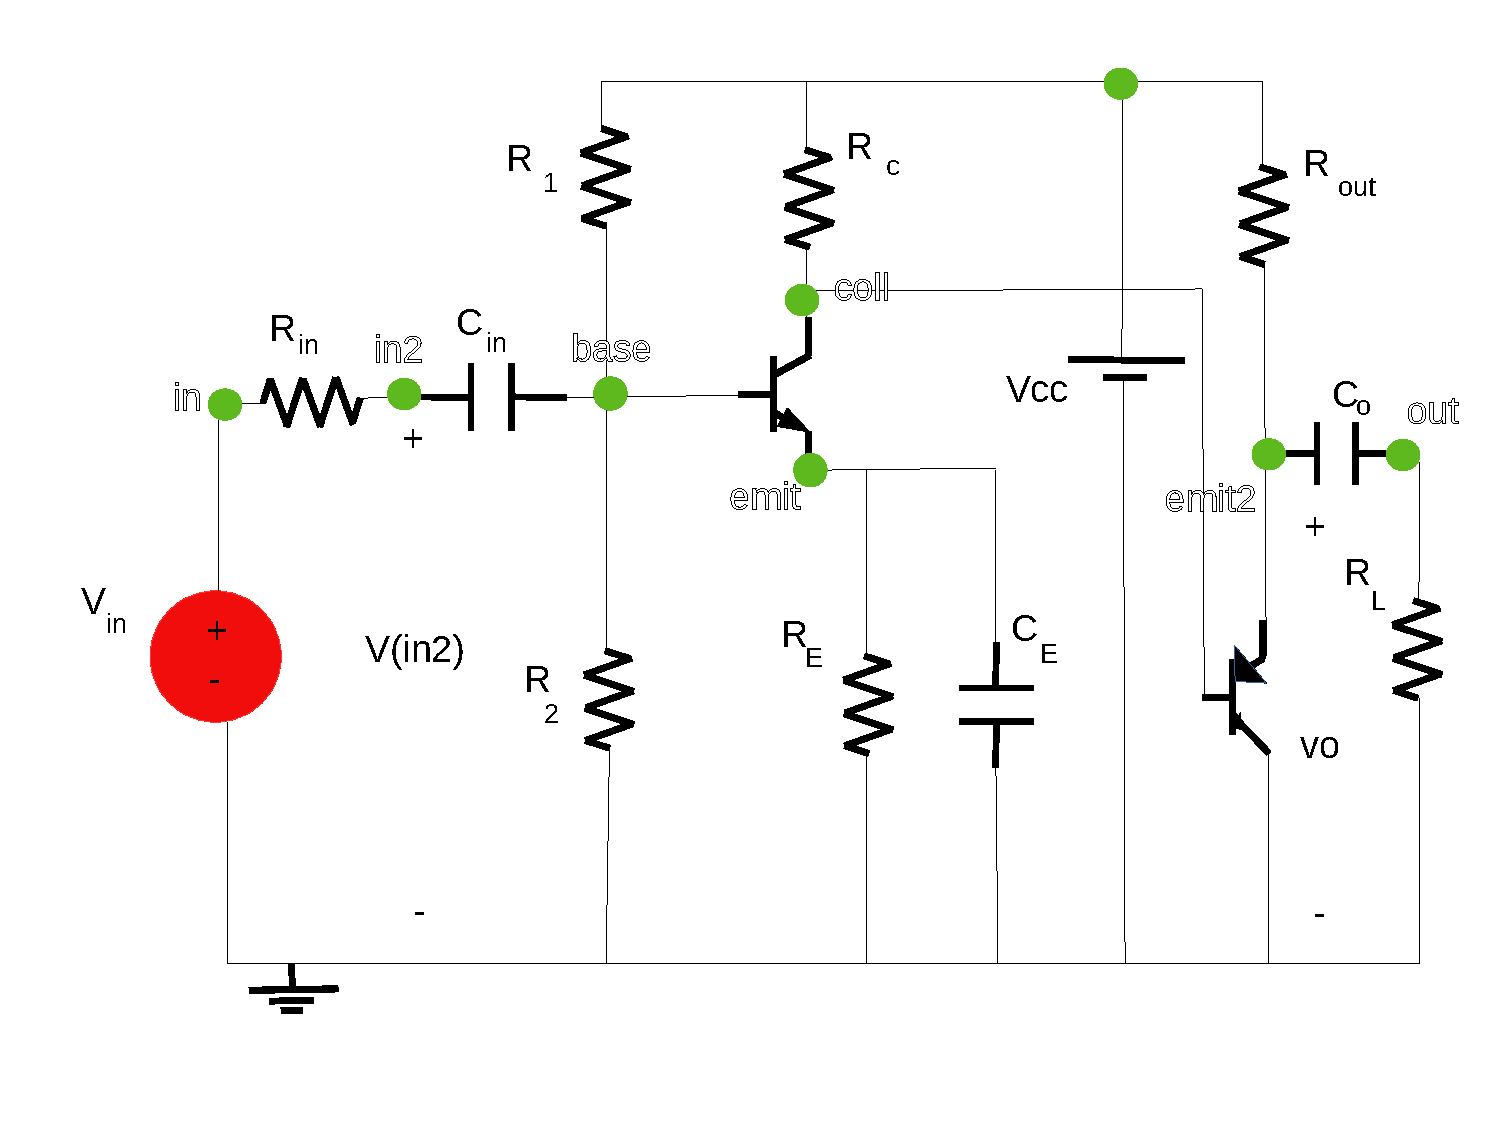
\includegraphics[width=0.5\linewidth]{lab4.pdf}
\caption{Circuit in analysis.}
\label{circuito todo}
\end{figure}


\begin{table}[ht]
  \centering
  \begin{tabular}{|l|r|}
    \hline    
    {\bf Name} & {\bf Value} \\ \hline
    Cin & 5.000000e-04 \\ \hline
CE & 5.000000e-04 \\ \hline
Cout & 2.000000e-04 \\ \hline
R1 & 2.000000e+04 \\ \hline
R2 & 2.000000e+03 \\ \hline
RC & 3.000000e+03 \\ \hline
RE & 1.000000e+02 \\ \hline
Rout & 1.000000e+02 \\ \hline
Vin & 1.000000e-02 \\ \hline
Vcc & 1.200000e+01 \\ \hline

  \end{tabular}
  \caption{Used Values of each component.}
  \label{tab:3}
\end{table}


\newpage


